\documentclass{beamer}

\usepackage[utf8]{inputenc}
\usepackage[brazil]{babel}
\usepackage{graphicx,hyperref,icmc,url}
\usepackage{subcaption}
\usepackage{multirow}
\usepackage{tikz}
\newcommand{\destaq}[1]{\textcolor{purple}{\textbf{#1}}}

% The title of the presentation:
%  - first a short version which is visible at the bottom of each slide;
%  - second the full title shown on the title slide;
\title[Reconstrução de curvas por características robustas extraídas de imagens]{Reconstrução de curvas por meio de características robustas extraídas de imagens}

% The author(s) of the presentation:
%  - again first a short version to be displayed at the bottom;
%  - next the full list of authors, which may include contact information;
\author[André Luís Mendes Fakhoury]{
    \Large{André Luís Mendes Fakhoury} \\ \medskip
    \small{\href{mailto:andrefakhoury@usp.br}{\nolinkurl{andrefakhoury@usp.br}}} \\ \bigskip
    \small{Orientador: João do Espirito Santo Batista Neto}
}

% \\ \bigskip
    % \large{}

% The institute:
%  - to start the name of the university as displayed on the top of each slide
%    this can be adjusted such that you can also create a Dutch version
%  - next the institute information as displayed on the title slide
\institute[ICMC/USP]{
    Vinculado ao Projeto Temático FAPESP: ``Mapeamento de características robustas entre diferentes domínios e espaços $\mathbb{R}^2$ e $\mathbb{R}^3$''\\ \medskip
    Instituto de Ciências Matemáticas e de Computação -- ICMC \\
    Universidade de São Paulo - USP
}

% Add a date and possibly the name of the event to the slides
%  - again first a short version to be shown at the bottom of each slide
%  - second the full date and event name for the title slide
\date[21/10/2021]{\footnotesize{21 de outubro de 2021}}

\AtBeginSection[]
{
    \begin{frame}<beamer>{Sumário}
        \tableofcontents[currentsection]
    \end{frame}
}

\begin{document}
    
    \begin{frame}[plain]
        \titlepage
    \end{frame}
    
    \begin{frame}
      \frametitle{Sumário}
      \tableofcontents
    \end{frame}
    
%%%%%%%%%%%%%%%%%%%%%%%%%%%%%%%%%%%%%%%%%%%%%%%%%%%%%%%%%%%%%%%%

\section{Introdução} % intro do projeto e objetivos
\begin{frame}
\frametitle{Contextualização}

\begin{itemize}
\item \destaq{Mapeamento} de características robustas entre espaços bidimensionais e tridimensionais;
\item Simplificação através da \destaq{redução} da quantidade de informações.
\end{itemize}

\end{frame}

\begin{frame}
\frametitle{Contextualização}

\destaq{Objetiva-se:}
\medskip
\begin{itemize}
	\item Pré-processar a imagem original;
	\item Extrair o contorno da figura;
	\item Extrair pontos importantes desta curva;	
	\item Reconstruir a curva original a partir destes pontos (características robustas).
\end{itemize}

\end{frame}



\section{Métodos e procedimentos} % diagrama de atividades realizadas
\begin{frame}
\frametitle{Métodos e Procedimentos}
\framesubtitle{Visão geral}

\begin{figure}[hbt]
	\begin{center}
		\caption{Diagrama de bloco das etapas de desenvolvimento}
		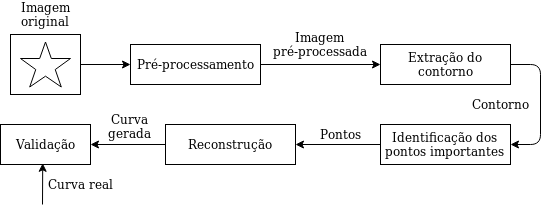
\includegraphics[width=1\textwidth]{img/diagrama.png}
	\end{center}
\end{figure}

\end{frame}

% pre processamento
\subsection{Pré-processamento}

\begin{frame}
\frametitle{Pré-processamento}

\destaq{Objetivos:}
\begin{itemize}
\item Suavizar a imagem
\item Remover ruídos
\end{itemize}

\bigskip
\destaq{Técnicas utilizadas:}
\begin{itemize}
	\item Filtro gaussiano ou Perona-Malik
	\item Binarização por Otsu
	\item Operadores morfológicos (erosão e dilatação)
\end{itemize}
\end{frame}

\begin{frame}
\frametitle{Pré-processamento}

\destaq{Extração do contorno:}
\begin{itemize}
	\item Acompanha a borda do objeto, e verifica se seus vizinhos também pertencem ao objeto.
\end{itemize}

\begin{figure}[hbt]
	\begin{center}
		\caption{Método \textit{contour following}~\cite{book_shape}}
		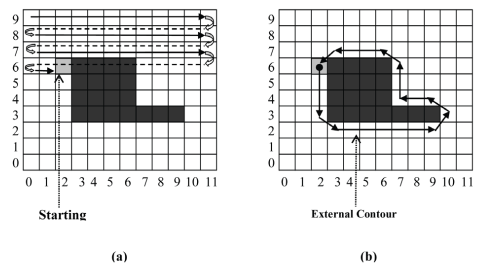
\includegraphics[width=0.6\textwidth]{img/contorno.png}
	\end{center}
\end{figure}
\end{frame}

% calculo da curvatura + contorno
\subsection{Curvatura}


% reconstrucao - sorkine
\subsection{Reconstrução}

\begin{frame}
\frametitle{Reconstrução}
\framesubtitle{Definições}

\destaq{Modelagem geométrica:} conjunto de técnicas e algoritmos utilizados para modelar determinadas formas matemáticas, sujeitas a condições particulares de forma e suavidade.


\medskip
Uma forma possível de se modelar é com a utilização do \destaq{operador discreto de Laplace-Beltrami} \cite{Sorkine2006}.

\end{frame}

\begin{frame}
\frametitle{Coordenadas diferenciais}

Seja uma malha triangular $\mathcal{M} = (V, E, F)$. Cada vértice $\mathbf{v}_i \in V$ possui uma representação cartesiana dada por $\mathbf{v}_i = (x_i,y_i,z_i)$.

\medskip

\destaq{Coordenadas diferenciais} (ou $\mathbf{\delta}$\textit{-coordenadas}) de $\mathbf{v}_i$ são definidas como a diferença entre a coordenada cartesiana e o centro de massa de seus vizinhos imediatos na malha:

\begin{equation}
	\mathbf{\delta}_i = (\mathbf{\delta}_i^{(x)}, \mathbf{\delta}_i^{(y)}, \mathbf{\delta}_i^{(z)}) = \mathbf{v}_i - \frac{1}{d_i} \sum_{j \in N(i)} \mathbf{v}_j,
	\label{eq_delta}
\end{equation}

\noindent em que $N(i) = \{j|(i,j) \in E$\} e $d_i = |N(i)|$.

\end{frame}

\begin{frame}
\frametitle{Coordenadas diferenciais}
\framesubtitle{Transformação para $\delta$-coordenadas}

Seja $A$ a matriz de adjacências da malha:

$$
A_{ij} = \begin{cases}
	1&(i, j) \in E\\
	0&\text{caso contrário.}
\end{cases}
$$

e $D$ a matriz diagonal tal que

$$D_{ii} = d_{i} = |N(i)| = \text{número de vértices adjacentes a }i$$

A matriz $L$ de transformação de coordenadas cartesianas para as coordenadas diferenciais é:

\begin{equation}
	L = I - D^{-1}A.
\end{equation}

\end{frame}

\begin{frame}
\frametitle{Coordenadas diferenciais}
\framesubtitle{Transformação para $\delta$-coordenadas}

É mais comum utilizar a versão simétrica de $L$, $L_s$, tal que:

$$L_s = DL = D - A$$

e cada célula pode ser calculada por:

\begin{equation}
	(L_s)_{ij} = \begin{cases}
		d_i&i=j\\
		-1&(i, j) \in E\\
		0&\text{caso contrário.}
	\end{cases}
\end{equation}


\end{frame}

\begin{frame}
\frametitle{Coordenadas diferenciais}
\framesubtitle{Transformação para $\delta$-coordenadas}

Temos:

$$L_s \textbf{x} = \delta^{(x)}$$
$$L_s \textbf{y} = \delta^{(y)}$$
$$L_s \textbf{z} = \delta^{(z)}$$

e $L_s$ é denominado \destaq{Laplaciano topológico} da malha $\mathcal M$.

\end{frame}

\begin{frame}
\frametitle{Coordenadas diferenciais}
\framesubtitle{Discretização de Laplace-Beltrami}

Se considerar $\mathcal{M}$ uma aproximação linear por partes de uma superfície suave,

$$\delta_i = \frac{1}{d_i} \sum_{j \in N(i)}(\mathbf{v_i} - \mathbf{v_j})$$

é uma discretização de

$$\frac{1}{|\gamma|} \int_{v \in \gamma} (v_i - v) dl(v)$$

em que $\gamma$ é uma curva de uma superfície fechada simples em volta de $v_i$ e $|\gamma|$ é o comprimento de $\gamma$.

\end{frame}

\begin{frame}
\frametitle{Coordenadas diferenciais}
\framesubtitle{Discretização de Laplace-Beltrami}

Sabe-se que:

$$\lim\limits_{|\gamma|\rightarrow 0} \frac{1}{|\gamma|} \int_{v \in \gamma} (v_i - v) dl(v) = - H(v_i) n_i$$

em que $H(v_i)$ é a curvatura média de $v_i$ e $n_i$ é a normal à superfície.

\medskip

Intuitivamente, as $\delta$-coordenadas \destaq{encapsulam a forma local da superfície}.

\end{frame}

\begin{frame}
\frametitle{Vantagens das $\delta$-coordenadas}
	\begin{itemize}
		\item Representam detalhes locais
		\begin{itemize}
			\item A direção aproxima o vetor normal;
			\item A norma aproxima a curvatura média;
		\end{itemize}
		\medskip
		\item Utilização de matrizes esparsas (economizam tempo/memória computacionalmente).
	\end{itemize}
\end{frame}

\begin{frame}
\frametitle{Reconstrução de $v_i$}
\framesubtitle{A partir das $\delta$-coordenadas}

$$L_s \textbf{x} = \delta^{(x)}$$

\begin{itemize}
	\item $\delta$-coordenadas são invariantes à translação;
	\item $L$ e $L_s$ são singulares;
	\item $\textbf{x} = L_s^{-1} \delta^{(x)}$ é \textbf{indefinido}.
	\item \textbf{Solução:} adicionar restrições de quem se conhece a localização.
	
\end{itemize}

\end{frame}


\begin{frame}
\frametitle{Reconstrução de $v_i$}
\framesubtitle{A partir das $\delta$-coordenadas}

$$L_s \textbf{x} = \delta^{(x)}$$

\begin{itemize}
	\item $rank(L) = n - k$, em que $k$ é o número de componentes;
	\item Fixar vértices $C = \{1, 2, \dots, m\}$, em que sabe-se $\{v_{C_1}, v_{C_2}, \dots, v_{C_m}\}$;
	\item Ou seja, adicionar restrições $v_{j} = c_j,\ j \in C$;
	\item Tornando o sistema \textit{full-rank}.
\end{itemize}

\end{frame}


\begin{frame}
\frametitle{Reconstrução de $v_i$}
\framesubtitle{A partir das $\delta$-coordenadas}

Fixar vértices $C = \{1, \dots, m\}$ em que sabe-se $\{v_{C_1}, v_{C_2}, \dots, v_{C_m}\}$:

\bigskip

$$\left(\frac{L}{I_{m\times m} | 0}\right) \textbf{x} = \begin{pmatrix}
	\delta^{(x)} \\
	c_{1:m}
\end{pmatrix}$$

\bigskip
E o mesmo para os outros vetores de coordenadas $\mathbf{y, z, \dots}$
\medskip

\smallskip

\end{frame}


\begin{frame}
\frametitle{Reconstrução de $v_i$}
\framesubtitle{A partir das $\delta$-coordenadas}


Inicialmente, tem-se:

\bigskip

\begin{center}
	\begin{tikzpicture}
		\filldraw[fill=olive!30!white, draw=black] (0,0) rectangle node{$L_s$} (2,2);
		\filldraw[fill=blue!30!white, draw=black] (2.1,0) rectangle node{$x$} (3.1,2);
		\draw (3.4, 0.95) -- (3.7, 0.95);
		\draw (3.4, 1.05) -- (3.7, 1.05);
		\filldraw[fill=purple!30!white, draw=black] (4,0) rectangle node{$\delta^{(x)}$} (6,2);
	\end{tikzpicture}
\end{center}

\bigskip
\medskip
\smallskip

\end{frame}

\begin{frame}
\frametitle{Reconstrução de $v_i$}
\framesubtitle{A partir das $\delta$-coordenadas}

Fixar vértices $C = \{1, \dots, m\}$ em que sabe-se $\{v_{C_1}, v_{C_2}, \dots, v_{C_m}\}$:

\bigskip

\begin{center}
	\begin{tikzpicture}
		\filldraw[fill=olive!30!white, draw=black] (0,0) rectangle node{$L_s$} (2,2);
		\filldraw[fill=olive!50!white, draw=black] (0,0) rectangle node{$I_c$} (2,-0.8);
		\filldraw[fill=blue!30!white, draw=black] (2.1,0) rectangle node{$x$} (3.1,2);
		\draw (3.4, 0.95) -- (3.7, 0.95);
		\draw (3.4, 1.05) -- (3.7, 1.05);
		\filldraw[fill=purple!30!white, draw=black] (4,0) rectangle node{$\delta^{(x)}$} (6,2);
		\filldraw[fill=purple!50!white, draw=black] (4,0) rectangle node{$v_c$} (6,-0.8);
	\end{tikzpicture}
\end{center}

\end{frame}

\begin{frame}
\frametitle{Reconstrução de $v_i$}
\framesubtitle{A partir das $\delta$-coordenadas}

Fixar vértices $C = \{1, \dots, m\}$ em que sabe-se $\{v_{C_1}, v_{C_2}, \dots, v_{C_m}\}$:

\bigskip

\begin{center}
	\begin{tikzpicture}
		\filldraw[fill=olive!40!white, draw=black] (0,-0.8) rectangle node{$\tilde{L}$} (2,2);
		\filldraw[fill=blue!30!white, draw=black] (2.1,0) rectangle node{$x$} (3.1,2);
		\draw (3.4, 0.95) -- (3.7, 0.95);
		\draw (3.4, 1.05) -- (3.7, 1.05);
		\filldraw[fill=purple!30!white, draw=black] (4,0) rectangle node{$\delta^{(x)}$} (6,2);
		\filldraw[fill=purple!50!white, draw=black] (4,0) rectangle node{$v_c$} (6,-0.8);
	\end{tikzpicture}
\end{center}


\end{frame}

\begin{frame}
\frametitle{Reconstrução de $v_i$}
\framesubtitle{A partir das $\delta$-coordenadas}

\begin{figure}
	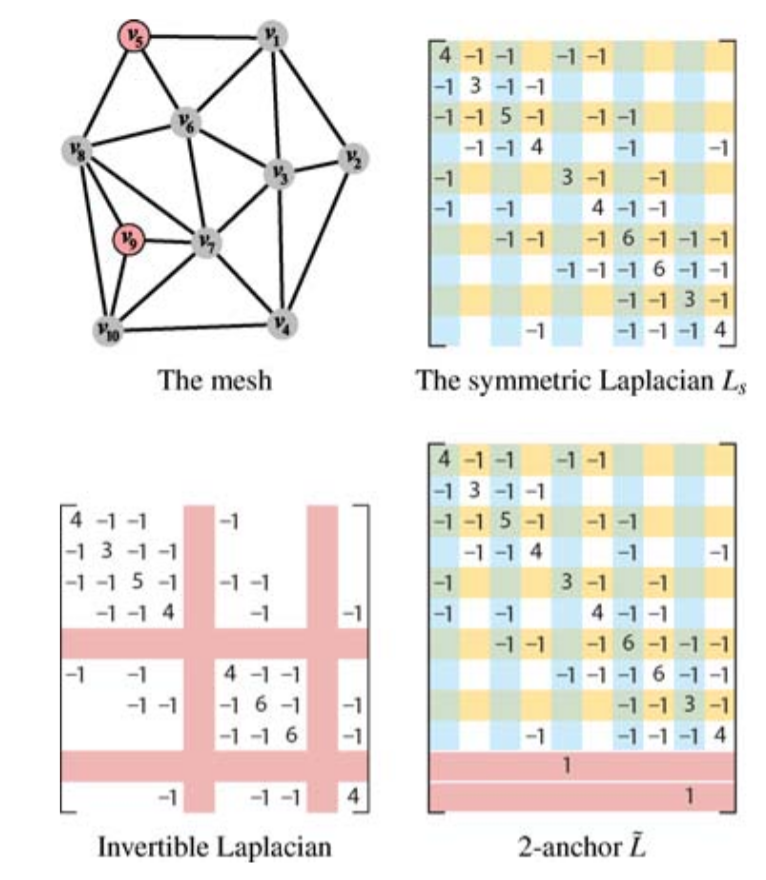
\includegraphics[width=0.5\linewidth]{img/lrestricao.png}
	\caption{Exemplo da matriz $\tilde{L}$ \cite{sorkine2006}}
\end{figure}
\end{frame}

\begin{frame}
\frametitle{Aplicações}
\framesubtitle{Representação eficiente de formas}

Com apenas informações de conectividade da malha e alguns pontos fixados (denominados vértices âncora), é possível aproximar toda a geometria, a partir da resolução do sistema pelo método dos mínimos quadrados:

\begin{equation}\label{eq:sisrecover}
	\left( \frac{L}{\omega I_{m \times m} | 0} \right) \mathbf{x'} = \begin{pmatrix}
		0\\
		\omega\ c_{1:m}^{(x)}
	\end{pmatrix}
\end{equation}

em que $c = \{v_1, v_2, \dots, v_m\}$ são os pontos âncora escolhidos como amostra, e $\omega > 0$ é o peso de cada restrição).

\end{frame}

\begin{frame}
\frametitle{Aplicações}
\framesubtitle{Representação eficiente de formas}

Graficamente, para facilitar a visualização, este sistema matricial também pode ser visto deste jeito:

\begin{center}
	\begin{tikzpicture}
		\filldraw[fill=olive!40!white, draw=black] (0,-0.8) rectangle node{$\tilde{L}$} (2,2);
		\filldraw[fill=blue!30!white, draw=black] (2.1,0) rectangle node{$x$} (3.1,2);
		\draw (3.4, 0.95) -- (3.7, 0.95);
		\draw (3.4, 1.05) -- (3.7, 1.05);
		\filldraw[fill=purple!30!white, draw=black] (4,0) rectangle node{$0$} (6,2);
		\filldraw[fill=purple!50!white, draw=black] (4,0) rectangle node{$v_c$} (6,-0.8);
	\end{tikzpicture}
\end{center}

\end{frame}


\begin{frame}
\frametitle{Aplicações}
\framesubtitle{Representação eficiente de formas}

Em vez de $\delta^{(x)}$ do lado direito, informa-se $0$ nas coordenadas em que não sabe a localização.

\medskip

Estas localizações serão calculadas por informações das malhas, descritas na matriz $\tilde{L}$.

\medskip

Por isso, é importante que se tenha conhecimento de informações de conectividade da malha em análise.
\end{frame}

\section{Resultados}
\begin{frame}
\frametitle{Resultados}

aiai imageclef curva 3d malhas sei la oq
	
\end{frame}


\begin{frame}
\frametitle{Resultados}
\framesubtitle{Imagens do banco de dados ImageCLEF (2011) \cite{imageclef2011}}

Coloca algumas folhas aqui

\end{frame}




\section{Conclusão}
\begin{frame}
\frametitle{Conclusão}

A utilização do \destaq{operador discreto de Laplace-Beltrami}:

\bigskip

\begin{itemize}
\item Permite boa reconstrução, se forem utilizados pontos âncora suficientes e escolhidos de maneira correta;
\item Alguns detalhes da malha original podem se perder, pois não serão considerados pelo algoritmo.
\end{itemize}

\end{frame}




%%%%%%%%%%%%%%%%%%%%%%%%%%%%
\section{Referências}

%\nocite{*}
\begin{frame}[allowframebreaks]
  \frametitle{Referência Bibliográfica}
  \bibliographystyle{siam}
  
  \bibliography{referencias}
\end{frame}

\end{document}
